%%
%% Author: Alexander Telich
%% 2/14/18
%%

% Preamble
\documentclass[11pt]{article}
\usepackage[utf8]{inputenc}
\usepackage{amsmath}

% Packages
\usepackage{a4wide}
\usepackage{listings}
\usepackage{indentfirst}
\usepackage{graphicx}

\lstdefinestyle{mystyle}{
basicstyle=\footnotesize,
breakatwhitespace=false,
breaklines=true,
captionpos=b,
keepspaces=true,
numbers=left,
numbersep=5pt,
showspaces=false,
showstringspaces=false,
showtabs=false,
tabsize=2
}

\lstset{style=mystyle}

\author{Alexander Telich}
\title{EECS 531 A1 Exercise 3}
\date{February 19, 2018}
\graphicspath{C:/Users/ateli/Documents/School/Spring 2018/EECS 531/Assignments/531_A1/A1/Exercise3}

% Document
\begin{document}
    \maketitle
    \section{Harris Corner Detection}\label{sec:exercise3}
    \subsection{Theory}\label{subsec:1.NoiseReduction}
    \setlength\parindent{24pt}
    The Harris Corner Detection technique essentially finds a difference in intensity for a displacement
    of $(u, v)$ in all directions.
    Basically it is a weighted sum of squared differences between two patches, the
    kernal matrix and the image pixel value matrix.
    This theory is denoted in equation (1).
    $w\left(x,\ y\right)$ is the 'window function' which gives weights to the pixels it is
    imposed onto. $I\left(x+u,\ y+v\right)$ is the shifted intensity of the function.
    $-I\left(x,\ y\right)$ is the intensity.
    \begin{equation}
        E\left(u,\ v\right)=\sum_{x,\ y}{w\left(x,\ y\right)\ \left[I\left(x+u,\ y+v\right)-I\left(x,\ y\right)\right]^2}
    \end{equation}
    \newline
    For this equation to detect corners the difference between the shifted intensity and the intensity squared
    must be maximized.
    This is denoted by equation (2).
    In this equation $I_x$ and $I_y$ are the derivatives of the image pixel values in the
    $x$ and $y$ directions, respectively.
    \begin{equation}
        M=\sum_{x,\ y}{w\left(x,y\right)\ \left[\begin{matrix}I_xI_x&I_xI_y\\I_xI_y&I_yI_y\\\end{matrix}\right]}
    \end{equation}
    \newline
    The final equation (3) gives the patch, or window, a score that determines whether or not it contains a corner.
    $det(M) = \lambda_1 \lambda_2$ and $trace(M) = {\lambda_1+\lambda_2}$. $\lambda_1$ and $\lambda_2$ are
    the Eigen values of the maximized equation (2).
    \begin{equation}
        R=\det{\left(M\right)}-k\left(trace\left(M\right)\right)^2
    \end{equation}

    \section{Code}\label{sec:codeExplanation}
    \lstinputlisting[language=Python]{Exercise3.py}

    \begin{figure}[h]
        \caption{Original Image}
        \centering
        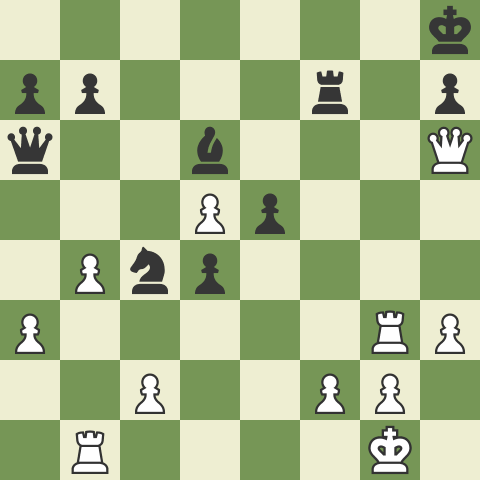
\includegraphics[scale=0.63]{dynboard.png}
    \end{figure}

    \begin{figure}[h]
        \caption{Image After Corners Detected}
        \centering
        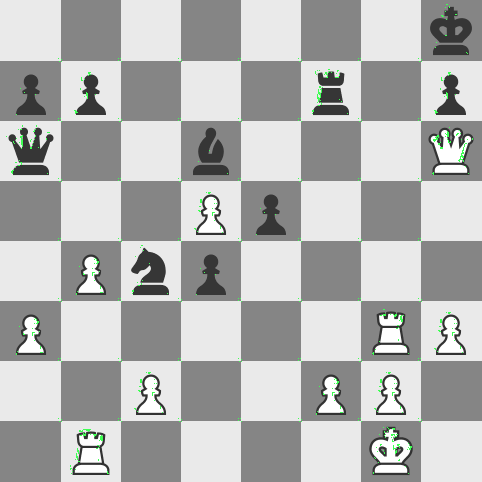
\includegraphics[scale=0.63]{Exercise3_OutputImage.png}
    \end{figure}

\end{document}
\begin{document}



\end{document}
\begin{document}



\end{document}